\documentclass[compress,blue]{beamer}

%\usepackage{beamerthemesplitcondensed}
\usepackage{beamertemplates}
\usepackage{beamerthemesplit}
\usepackage{beamerthemeshadow}
\usepackage[german]{babel}
\usepackage{pgf,pgfarrows,pgfnodes,pgfautomata,pgfheaps,pgfshade}
\usepackage{amsmath,amssymb}
\usepackage[latin1]{inputenc}
\usepackage{colortbl}
\usepackage{listings}
\usepackage{graphicx}
\usepackage{alltt}
\usepackage[T1]{fontenc}
\usepackage{ae,aecompl}

%\DeclareFontFamily{T1}{cmvtt}{}

\pgfdeclareimage[height=1cm]{unilogo}{logomitte}

\hypersetup{%
  pdftitle={Tracing von (Open-Source) Projekten mit Maven},%
  pdfauthor={Tammo van Lessen, Steffen Pingel},
  pdfsubject={inf.misc},
  pdfkeywords={Maven, Project Tracing, statcvs, xnap}}

\title[How to Mavenize your project]{Tracing von (Open-Source) Projekten mit Maven}
\author{Tammo van Lessen, Steffen Pingel}
\institute[Univerit�t Stuttgart]{
  Fakult�t f�r Elektrotechnik und Informatik\\
  Universit�t Stuttgart\\
  \vspace{0.5cm}
  \pgfuseimage{unilogo}\\
  \vspace{0.5cm}
  Fachgruppe IT Projekt-Management\\
  \vspace{0.5cm}
  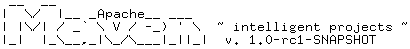
\includegraphics[height=1cm]{mavenlogo}
}
\date[inf.misc 2004]{inf.misc, 04.02.2004}

%\logo{\pgfuseimage{unilogo}}

%\definecolor{structure}{rgb}{0.282, 0.243, 0.443}

\beamertemplateshadingbackground{red!10}{structure!10}
%\beamertemplatetransparentcovereddynamic
\beamertemplatetransparentcovered
%\beamertemplateballitem

\definecolor{korange}{rgb}{0.964, 0.631, 0.109}

  \pgfdeclareradialshading{bigsphere}{\pgfpoint{-0.9pt}{1.1pt}}%
  {color(0cm)=(korange!15);
    color(0.8pt)=(korange!75);
    color(1.6pt)=(korange!70!black);
    color(2.2pt)=(korange!50!black);
    color(2.6pt)=(averagebackgroundcolor)}
  \pgfdeclareradialshading{smallsphere}{\pgfpoint{-0.72pt}{0.89pt}}%
  {color(0cm)=(korange!15);
    color(0.64pt)=(korange!75);
    color(1.28pt)=(korange!70!black);
    color(1.76pt)=(korange!50!black);
    color(2.08pt)=(averagebackgroundcolor)}
  
  \begin{colormixin}{20!averagebackgroundcolor}
  \pgfdeclareradialshading{bigsphereshaded}{\pgfpoint{-0.9pt}{1.1pt}}%
  {color(0cm)=(korange!15);
    color(0.8pt)=(korange!75);
    color(1.6pt)=(korange!70!black);
    color(2.2pt)=(korange!50!black);
    color(2.6pt)=(averagebackgroundcolor)}
  \pgfdeclareradialshading{smallsphereshaded}{\pgfpoint{-0.72pt}{0.89pt}}%
  {color(0cm)=(korange!15);
    color(0.64pt)=(korange!75);
    color(1.28pt)=(korange!70!black);
    color(1.76pt)=(korange!50!black);
    color(2.08pt)=(averagebackgroundcolor)}
  \end{colormixin}
  \pgfaliasshading{bigsphere!20!averagebackgroundcolor}{bigsphereshaded}
  \pgfaliasshading{smallsphere!20!averagebackgroundcolor}{smallsphereshaded}
  
  \begin{colormixin}{15!averagebackgroundcolor}
  \pgfdeclareradialshading{bigsphereshaded}{\pgfpoint{-0.9pt}{1.1pt}}%
  {color(0cm)=(korange!15);
    color(0.8pt)=(korange!75);
    color(1.6pt)=(korange!70!black);
    color(2.2pt)=(korange!50!black);
    color(2.6pt)=(averagebackgroundcolor)}
  \pgfdeclareradialshading{smallsphereshaded}{\pgfpoint{-0.72pt}{0.89pt}}%
  {color(0cm)=(korange!15);
    color(0.64pt)=(korange!75);
    color(1.28pt)=(korange!70!black);
    color(1.76pt)=(korange!50!black);
    color(2.08pt)=(averagebackgroundcolor)}
  \end{colormixin}
  \pgfaliasshading{bigsphere!15!averagebackgroundcolor}{bigsphereshaded}
  \pgfaliasshading{smallsphere!15!averagebackgroundcolor}{smallsphereshaded}
  
  \begin{colormixin}{10!averagebackgroundcolor}
  \pgfdeclareradialshading{bigsphereshaded}{\pgfpoint{-0.9pt}{1.1pt}}%
  {color(0cm)=(korange!15);
    color(0.8pt)=(korange!75);
    color(1.6pt)=(korange!70!black);
    color(2.2pt)=(korange!50!black);
    color(2.6pt)=(averagebackgroundcolor)}
  \pgfdeclareradialshading{smallsphereshaded}{\pgfpoint{-0.72pt}{0.89pt}}%
  {color(0cm)=(korange!15);
    color(0.64pt)=(korange!75);
    color(1.28pt)=(korange!70!black);
    color(1.76pt)=(korange!50!black);
    color(2.08pt)=(averagebackgroundcolor)}
  \end{colormixin}
  \pgfaliasshading{bigsphere!10!averagebackgroundcolor}{bigsphereshaded}
  \pgfaliasshading{smallsphere!10!averagebackgroundcolor}{smallsphereshaded}
  
  \begin{colormixin}{5!averagebackgroundcolor}
  \pgfdeclareradialshading{bigsphereshaded}{\pgfpoint{-0.9pt}{1.1pt}}%
  {color(0cm)=(korange!15);
    color(0.8pt)=(korange!75);
    color(1.6pt)=(korange!70!black);
    color(2.2pt)=(korange!50!black);
    color(2.6pt)=(averagebackgroundcolor)}
  \pgfdeclareradialshading{smallsphereshaded}{\pgfpoint{-0.72pt}{0.89pt}}%
  {color(0cm)=(korange!15);
    color(0.64pt)=(korange!75);
    color(1.28pt)=(korange!70!black);
    color(1.76pt)=(korange!50!black);
    color(2.08pt)=(averagebackgroundcolor)}
  \end{colormixin}
  \pgfaliasshading{bigsphere!5!averagebackgroundcolor}{bigsphereshaded}
  \pgfaliasshading{smallsphere!5!averagebackgroundcolor}{smallsphereshaded}
  
  \begin{colormixin}{2!averagebackgroundcolor}
  \pgfdeclareradialshading{bigsphereshaded}{\pgfpoint{-0.9pt}{1.1pt}}%
  {color(0cm)=(korange!15);
    color(0.8pt)=(korange!75);
    color(1.6pt)=(korange!70!black);
    color(2.2pt)=(korange!50!black);
    color(2.6pt)=(averagebackgroundcolor)}
  \pgfdeclareradialshading{smallsphereshaded}{\pgfpoint{-0.72pt}{0.89pt}}%
  {color(0cm)=(korange!15);
    color(0.64pt)=(korange!75);
    color(1.28pt)=(korange!70!black);
    color(1.76pt)=(korange!50!black);
    color(2.08pt)=(averagebackgroundcolor)}
  \end{colormixin}
  \pgfaliasshading{bigsphere!2!averagebackgroundcolor}{bigsphereshaded}
  \pgfaliasshading{smallsphere!2!averagebackgroundcolor}{smallsphereshaded}
  \pgfaliasshading{bigsphere!20!averagebackgroundcolor,15!averagebackgroundcolor}{bigsphereshaded}
  \pgfaliasshading{bigsphere!15!averagebackgroundcolor,15!averagebackgroundcolor}{bigsphereshaded}
  \pgfaliasshading{bigsphere!10!averagebackgroundcolor,15!averagebackgroundcolor}{bigsphereshaded}
  \pgfaliasshading{bigsphere!5!averagebackgroundcolor,15!averagebackgroundcolor}{bigsphereshaded}
  \pgfaliasshading{bigsphere!2!averagebackgroundcolor,15!averagebackgroundcolor}{bigsphereshaded}  
  \pgfaliasshading{smallsphere!20!averagebackgroundcolor,15!averagebackgroundcolor}{smallsphereshaded}
  \pgfaliasshading{smallsphere!15!averagebackgroundcolor,15!averagebackgroundcolor}{smallsphereshaded}
  \pgfaliasshading{smallsphere!10!averagebackgroundcolor,15!averagebackgroundcolor}{smallsphereshaded}
  \pgfaliasshading{smallsphere!5!averagebackgroundcolor,15!averagebackgroundcolor}{smallsphereshaded}
  \pgfaliasshading{smallsphere!2!averagebackgroundcolor,15!averagebackgroundcolor}{smallsphereshaded}
  
  \useitemizeitemtemplate{\raise0.2pt\hbox{\pgfuseshading{bigsphere}}}
  \usesubitemizeitemtemplate{\raise0.2pt\hbox{\pgfuseshading{smallsphere}}}


%  \useitemizeitemtemplate{\small\raise0.5pt\hbox{\color{korange}\textbullet}}
%  \usesubitemizeitemtemplate{\footnotesize\raise0.5pt\hbox{\color{structure}\textbullet}}


\beamertemplatesolidbuttons
\beamertemplateroundedblocks
\beamertemplatelargetitlepage

\begin{document}

\plainframe[all:1]{\titlepage}

\section[Outline]{}
\frame{
  \begin{enumerate}
  \item Project Tracing und Entwicklungsphilosophien
  \item Basics
  \item Plugins
  \item Advanced Stuff
  \item Fazit
  \end{enumerate}
}

\part{Project Tracing}
\plainframe{\partpage}
\section[Tracing]{Project Tracing}
% \frame{
%     \frametitle{Verfolgung von Projekten}
%     Tracing ist bestandteil der Dokumentation von Projekten. Prozessdoku.
%     OpenSource: Erfolgreiche OS-Projekte brauchen 4 Dinge: Projekt, Code, Dokumentation, Community.
%     Apache Way of Life.
%     H�ufigster Fehler: keine Doku.
%     Lehrbuchmodell: schreibt die Dokumentation schon vor.
%     Dokumentation ist aufwendig, deshalb automatisieren.
% }

% \frame{
%     \frametitle{Erfolgreiche Projekte}
%     Erfolgreiche Projekte brauchen 4 Dinge:
%     \begin{itemize}
%         \item das Projekt (bildet den Rahmen)
%         \item den Quellcode (klar!)
%         \item \alert<2>{ausf�hrliche Dokumentation (!!)}
%         \item eine Community / einen Kunden.
%     \end{itemize}
%     \vspace{0.5cm}
%     \invisible<1>{Zur Dokumentation geh�ren
%     \begin{itemize}
%         \item Beschreibung der Schnittstellen (API Dokumentation)
%         \item Ergebnisse der Unit-Tests inkl. Messung der Test�berdeckung
%         \item Erhebung und Visualisierung von Metriken
%         \item Produktdokumentation (Handb�cher, Online-Hilfe etc.)
%     \end{itemize}}
% }

% \frame{
%     \frametitle{Automatisierter Buildprozess}
%     Autmatisches Build gr��erer Projekte mit Ant und Make.
%     Nachteile:
%     \begin{itemize}
%         \item{Targets k�nnen nicht zwischen Projekten geteilt werden}
%         \item{Builddateien fast identisch}
%         \item{Kein Scripting m�glich (keine Loops/Conditionals)}
%         \item{Verwendung von 3rd-Party-Tools (z.B. javadoc) relativ umst�ndlich}
%         \item{Keine Aufl�sung von Library-Dependencies (Jar-H�lle)}
%     \end{itemize}
%     \vspace{0.5cm}
%     \large{\bf{L�sung:} Apache Maven}
% }


\frame{
    \frametitle{Project Tracing}
    \begin{block}{Ziel}
        Die Entwicklung bestimmter Projektparameter zu verfolgen.
        Wo steht mein Projekt jetzt in diesem Moment?
    \end{block}
    
    \begin{itemize}
        \item BWL-Sicht: Zeit, Resourcen, Kosten, Umfang
        \item Entwickler-Sicht: Qualit�t, Velocity, gute Dokumentation, Source-Metriken...
    \end{itemize}
}

\frame{
    \frametitle{Anatomie (eines Open-Source-Projekts)}
    \begin{columnsonlytextwidth}
    \begin{column}{5cm}
    \begin{itemize}
        \item Projekt ist ''nur'' die H�lle
        \item Eigentlicher Kern \begin{itemize}
            \item Code
            \item Dokumentation
            \item Community (Kunde)
        \end{itemize}
        \item Ohne diese 4 kann ein Projekt nicht erfolgreich sein.
    \end{itemize}
    \end{column}
    \begin{column}{5cm}
    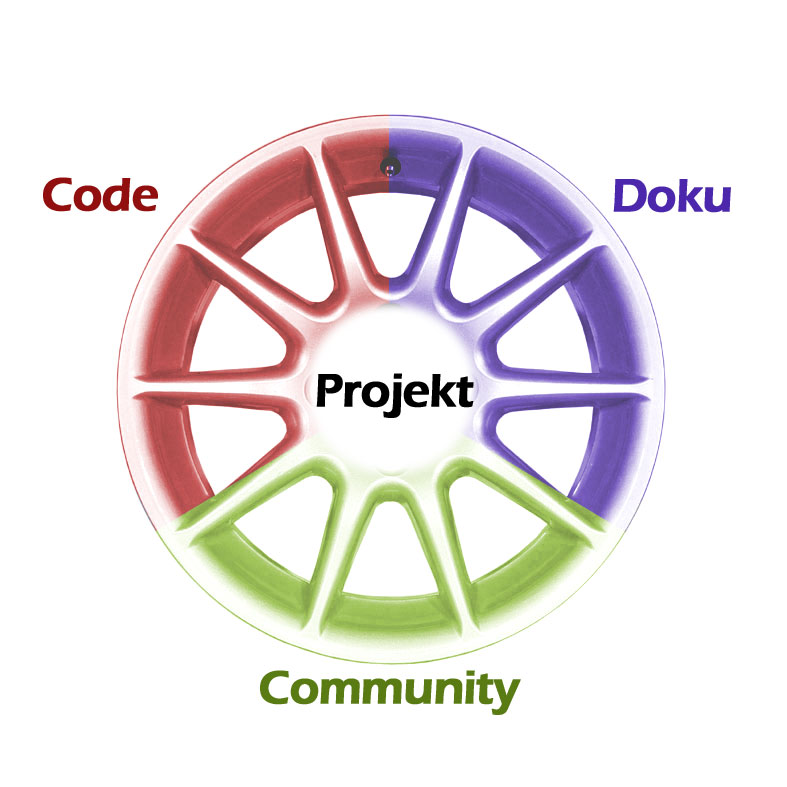
\includegraphics[width=5cm]{cdc}
    \end{column}
    \end{columnsonlytextwidth}
}

\frame{
    \frametitle{Project Tracing (in Open-Source-Projekten)}
    
    \begin{itemize}
        \item Einheitliche Dokumentation
        \item Architektur sichtbar machen
        \item Wer hat als letztes Was Wo gemacht? (Collective File Ownership)
        \item Qualit�tssicherung durch Source-Metriken
        \item Test�berdeckung
        \item �berblick �ber die verwendeten Bibliotheken
    \end{itemize}
    
    Das alles, und noch viel mehr: Automatisch im Buildprozess. Mit {\bf Apache Maven}.
}



\part{Maven Basics}
\plainframe{\partpage}
\section{Einfuehrung}
\subsection{Hintergrund}
%Maven was initially developed for buiding Turbine, Maven matured into an open source software engineering platform, The core functionality is automated project building, distribution and website creation 
%an easy way to publish project information and a way to share JARs across several projects.

\section{Installation}
\frame{
maven genapp
Verzeichnisstruktur
}
\section{Konzepte}
% 3 Kerndateien
% TARGET=GOAL (post/preGoal)
%A project is described with
%a XML Project Object
%Model (POM)
% The POM defines how to
%build a project and the
%external dependencies
% The Maven functionality is
%implemented in terms of
%plugins
% The plugins are written in
%Jelly
% JARs are downloaded
%from a remote repository
%and stored into a local
%repository
\subsection{Architektur}
%grafik
\subsection[POM]{Project Object Model}
% projekt eigenschaften
\subsection[PP]{Project Properties}
% customizing von plugins
\subsection{Repositories}

\section{Beispiel}

%%% Local Variables: 
%%% TeX-master: "index"
%%% End: 


\part{Maven Plugins}
\plainframe{\partpage}
\section{Core Plugins}

\subsection{�bersicht}
\frame{
  \frametitle{�bersicht}

  Die Core Plugins werden mit Maven ausgeliefert. Einige kennen wir bereits:
  
  \begin{itemize}
  \item clean
  \item jar
  \item java
  \end{itemize}

}

\subsection{ChangeLog}
\frame{
  \frametitle{ChangeLog Plugin}
}

\subsection{License}
\frame{
  \frametitle{License Plugin}
}

\section{Optional Plugins}

\subsection{�bersicht}
\frame{
  \frametitle{�bersicht}

  Die Optionalen Plugins werden bei Bedarf automatisch
  installiert. Auch hier haben wir einige bereits gesehen:

  \begin{itemize}
  \item genapp
  \item linkcheck
  \item release
  \item site
  \item xdoc
  \end{itemize}

  Auf der Maven Seite sind Ende Januar 2004 77 Plugins gelistet.
}

\subsection{Changes}
\frame{
  \frametitle{Changes Plugin}

  Versions Historie

  changes.xml
}

\subsection{Source Code Dokumentation}
\frame{
  \frametitle{Source Code Dokumentation}
  
  JavaDoc
  XRef
  JUnit
}

\subsection{Source Code Metriken}
\frame{
  \frametitle{Source Code Metriken}
  
   CheckStyle Plugin
   PMD Plugin
}

\subsection{Test�berdeckung}
\frame{
  \frametitle{Test�berdeckung}
  
   Clover
   JCoverage
   gcover
}

\subsection{CVS Statistiken}
\frame{
  \frametitle{CVS Statistiken}

  Developer Activity Plugin
  File Activity Plugin
}

\frame{
  \frametitle{StatCvs Plugin}
}

\subsection{Weitere}
\frame[all:1]{
  \frametitle{Noch Mehr N�tliche Plugins}

  \begin{itemize}
  \item ant
  \item console: Konsoleneingabe zum Aufruf von Goals
    \begin{itemize}
    \item (+) schnelles sukessives Aufrufen von Goals
    \item (-) unzureichende Speicherfreigabe f�hrt zu OutOfMemory
      exception
    \end{itemize}
  \item eclipse: Generierung von Eclipse Projekt Dateien
    \begin{itemize}
    \item Ber�cksichtigung aller Dependencies
    \item Anlegen der MAVEN\_HOME Variable in Eclipse notwendig
    \end{itemize}
  \item plugin
  \item release
  \item uberjar
  \end{itemize}
}


%%% Local Variables: 
%%% TeX-master: "index"
%%% End: 


\part{Beyond the Basics}
\plainframe{\partpage}
\section[Tipps]{Tipps}

\subsection{Command Line}

\frame[all:1]{
  \frametitle{Command Line Optionen}
  
  \begin{itemize}
  \item \begin{alltt}-g\end{alltt} Eine Liste aller Goals anzeigen
  \item -o Offline Modus. Nur Goals ausf�hren, die keine Internet
    Verbindung ben�tigen
  \item -p Project Datei angeben. N�tzlich f�r aufrufe aus nicht Projekt
    Verzeichnissen (z.B. in einem cron job).
  \end{itemize}
}

\subsection{Konfiguration}

\frame[all:1]{
  \frametitle{Konfiguration}
  
  Pers�nliche Einstellungen k�nnen in \$HOME/build.properties
  vorgenommen werden.

  \begin{alltt}
    maven.repo.local=/usr/local/maven-1.0-rc1/repository
    maven.home.local=/usr/local/maven-1.0-rc1
    java.compiler=modern
    maven.username=nick
  \end{alltt}
}

\frame[all:1]{
  \frametitle{Customizing}
  
  \begin{itemize}
  \item Jelly: Code und Layout bunt durcheinander gemischt
  \item xnap.jsl Ein Beispiel f�r ein 3 Column Layout
  \item Includieren von php Skripten 
  \end{itemize}

\begin{alltt}
<jsl:template match="include" trim="false">
  <x:set var="_file" select="string(@file)"/>
  <jsl:comment>#include virtual="${_file}"</jsl:comment>
</jsl:template>
\end{alltt}

\begin{alltt}
<section name="FAQ">
<p><include file="faq.php"/></p>
\end{alltt}

}

%%% Local Variables: 
%%% TeX-master: "index"
%%% End: 


\part{Fazit}
\plainframe{\partpage}
\section{Zusammenfassung}

\frame{
  \frametitle{Zusammenfassung}

  \begin{columns}
    %\begin{column}{6cm}
	\begin{minipage}[t]{6cm}
  Maven ist ein {\bf brauchbares} Tool
  
  \begin{itemize}
  \item Sehr einfache Erstellung von Projektdokumentation
  \item Sehr einfache Erhebung von Projekt- und Prozess-Metriken
  \item Sehr einfaches Building und Releasing, Deploying 
  \item Automatische Aufl�sung von Abh�ngigkeiten
  \end{itemize}  
    \end{minipage}
    \begin{minipage}[t]{6cm}
  Manches ist noch {\bf nicht ausgereift}

  \begin{itemize}
  \item Lange Startzeiten (auf marvin ca. 4s)
  \item Viele Reports sind Java spezifisch
  \item Anpassung der Webseiten schwierig
  \item Keine I18n Unterst�tzung
  \item Generierte Webseiten enthalten viele Leerzeilen
  \item Aufruf aus ``falschen'' Verzeichnissen f�hrt zu {\it sehr} wirren Meldungen
  \end{itemize}
    \end{minipage}
  \end{columns}
}
  
\subsection{Resourcen}
\frame{
  \frametitle{Resourcen}

  \begin{itemize}
  \item http://maven.apache.org/
  \item http://maven.apache.org/reference/plugins/index.html
  \item http://jakarta.apache.org/commons/jelly/
  \item http://maven-plugins.sourceforge.net/
  \item http://wiki.codehaus.org/maven/
  \end{itemize}
}

%%% Local Variables: 
%%% TeX-master: "index"
%%% End: 


\plainframe{
\Huge{Vielen Dank!}
}

\end{document}
